\section{Celda Sedra-Ghorab-Martin}

\subsection{Introducci\'on}
En este apartado se realiza un an\'alisis de la celda denominada Sedra-Ghorab-Martin, y posteriormente el dise\~no, s\'intesis y an\'alisis de un filtro activo empleando dicha celda. La principal fuente de informaci\'on ser\'a el paper denominado "\textit{Optimum configurations for Single-Amplifier Biquadratic Filters}"

\subsection{La celda Sedra-Ghorab-Martin}

La celda Sedra-Ghorab-Martin (en adelante, "celda SGB") es un circuito creado en el a\~no 1980 por los miembros de IEEE cuyos nombres se reflejan en el nombre de la celda. Dicho circuito se basa en el circuito pasabanda de Deliyannis, que se reproduce a continuaci\'on.

\begin{figure}[H] \label{fig:EJ3_deliyannis}
    \centering
    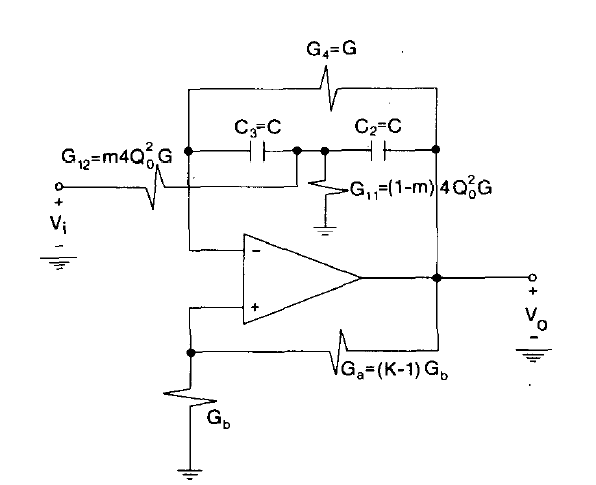
\includegraphics[width=0.8\textwidth]{../EJ3/Resources/deliyannis_cell.png}
    \caption{Pasabanda Deliyannis}
\end{figure}

Donde $k$ es una constante que es directamente proporcional a la cantidad de realimentaci\'on positiva del circuito.

Este circuito es posteriormente generalizado por Friend para poder construir cualquier tipo de configuraci\'on de filtro. El mismo se caracteriza por poseer una alta selectividad, empleando tanto realimentaci\'on positiva como negativa. Sin embargo, para poder sintetizar cualquier tipo de filtro es necesario cargar la red RC que se observa en la realimientaci\'on negativa del circuito~\ref{fig:EJ3_deliyannis}, lo que hace poco realizable el dise\~no del mismo.\\


Por otro lado, se encontr\'o que realizando una transformaci\'on complementaria sobre el circuito de Deliyannis (esto es, intercambiando la salida del amplificador operacional por masa, y procediendo an\'alogamente con la entrada inversora y no inversora del mismo) se deriva en el circuito de Sallen-Key manteniendo una realimentaci\'on positiva. Cabe destacar que esta transformaci\'on conserva la sensibilidad de los polos del circuito, pero no as\'i con los ceros de transmisi\'on del mismo. A\'un asi, se lleg\'o a la conclusi\'on de que es m\'as ventajoso implementar las configuraciones de filtros en una celda Sallen-Key con realimentaci\'on positiva (exceptuando el caso de un filtro pasabanda).\\


En la figura de abajo se observa como aplicando transformaci\'on complementaria y cambios en la red RC se llega a distintos circuitos con la caracter\'istica de poseer una red de realimentaci\'on similares a un circuito Sallen-Key.

\begin{figure}[H] \label{fig:EJ3_transformation_circuits}
    \centering
    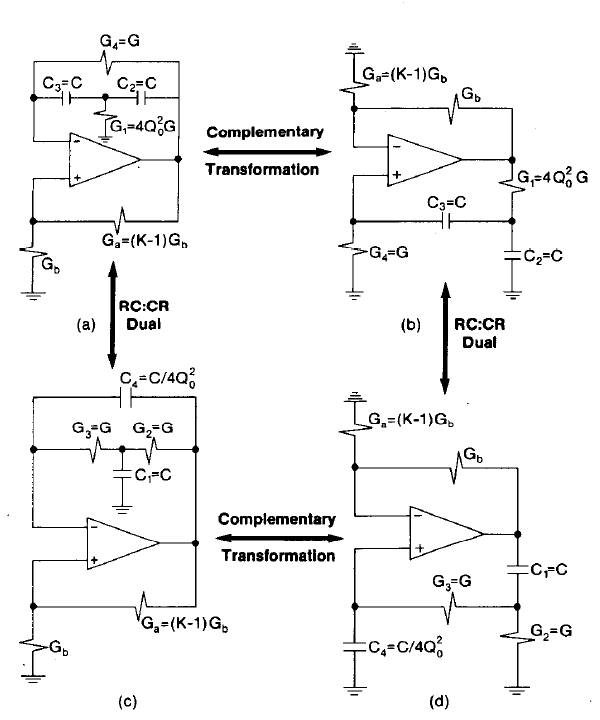
\includegraphics[width=0.7\textwidth]{../EJ3/Resources/transformation_circuits.png}
    \caption{Resultados de las transformaciones}
\end{figure}

Los circuitos \ref{fig:EJ3_transformation_circuits} b) y \ref{fig:EJ3_transformation_circuits} d) son llamados EPF (Enhanced positive feedback), y son la base de la celda SGB. Esta caracter\'istica esta dada por un coeficiente $K>1$. Para los cuatro circuitos de la figura se cumplen las siguientes ecuaciones que describen el comportamiento de los mismos.

\begin{equation}\label{EJ3eq1}
\frac{C}{G} = \frac{2Q_0}{\omega_0}
\end{equation}

\begin{equation}\label{EJ3eq2}
K-1 = \frac{1}{2Q_0^2}\cdot \left( 1-\frac{Q_0}{Q} \right)
\end{equation}

Donde $Q_0$ es un par\'ametro de dise\~no que cumple $Q>Q_0$. De esta forma, los circuitos del tipo EPF permiten implementar filtros con la siguiente funci\'on transferencia de segundo orden

\begin{equation}
H(s)=\frac{n_2s^2+n_1s+n_0}{s^2+s\left(\frac{\omega_0}{Q}\right)+\omega_0^2}
\end{equation}

Donde los coeficientes $n_i$ determinan los ceros de transmisi\'on, y por ende el tipo de filtro implementado por el circuito. Para poder lograr esto sin afectar la ubicacion de los polos se necesita que aquellos componentes que se encuentren conectados a masa sean desconectados de la misma, total o parcialmente (dividi\'endolos). Asi, se obtienen los dos circuitos HPB (\textit{high-pass biquad}) y LPB (\textit{low-pass biquad})que se muestran en las figuras \ref{EJ3_HPB} y \ref{EJ3_LPB} respectivamente.

\begin{figure}[H]
    \centering
    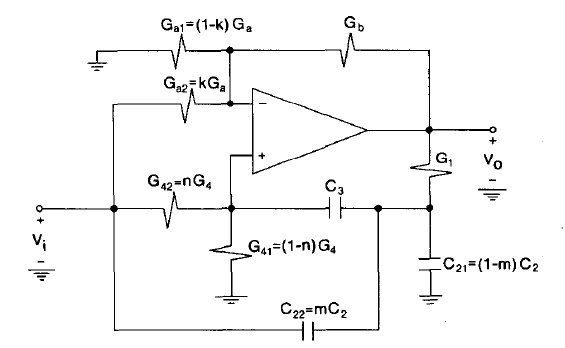
\includegraphics[width=0.7\textwidth]{../EJ3/Resources/HPB.png}
    \caption{High-pass biquad}
     \label{EJ3_HPB}
\end{figure}

\begin{figure}[H] 
    \centering
    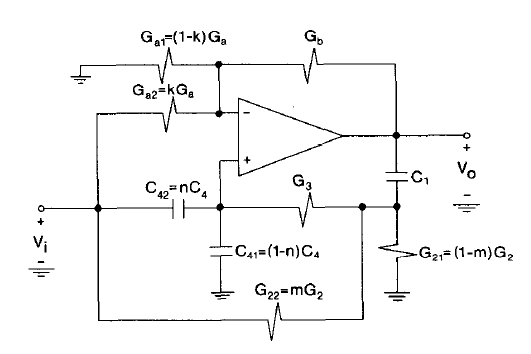
\includegraphics[width=0.7\textwidth]{../EJ3/Resources/LPB.png}
    \caption{Low-pass biquad}
    \label{EJ3_LPB}
\end{figure}

Como sus nombres lo indican, ambos circuitos son empleados para la implementaci\'on de distintos tipos de filtros. El circuito a elegir en funci\'on de la aplicaci\'on elegida se muestra en la tabla a continuaci\'on.

\begin{table}[H]
    \centering
    \begin{tabular}{c c}
        Tipo de Filtro & Circuito Recomendado \\
        \hline
        Pasabajos & LPB (fig.~\ref{EJ3_LPB}) \\
        Pasaaltos & HPB (fig.~\ref{EJ3_HPB}) \\
        Pasabanda & Deliyannis (fig.~\ref{fig:EJ3_deliyannis}) \\
        Pasatodo & LPB o HPB \\
        High pass notch & HPB \\
        Low pass notch & LPB\\
    \end{tabular}
    \caption{Circuitos recomendados}
    \label{tabla_circuitos}
\end{table}

\todo{Seguir con el desarrollo de la celda. Poner ecuaciones de equivalencias de coeficientes, y analizar sensibilidades (todo en forma gen\'erica y para HPB y LPB solamente)}

\subsection{Implementaci\'on de filtro}
Realizado el an\'alisis de la celda en cuesti\'on, se pide implementar un filtro pasaaltos activo con la misma, que cumpla con las condiciones fijadas en la tabla~\ref{tabla_filtro}.

\begin{table}[H]
    \centering
    \begin{tabular}{c c c}
        Par\'ametro & Valor indicado & Valor efectivo \\
        \hline
         $f_a$ & $\left( 10+1,1\cdot \frac{N}{2} \right) kHz$  & $10,55 kHz$  \\
         $f_p$ & $2 \cdot f_a $ & $21,1kHz$  \\
         $A_p$ & $2dB$ & $2dB$ \\
         $A_a$ & $40dB$ & $40dB$  \\
         $Z_{in}$ & $>50k\Omega$ & $>50k\Omega$  \\
    \end{tabular}
    \caption{Especificaciones del filtro}
    \label{tabla_filtro}
\end{table}

El primer paso para el dise\~no del mismo es normalizar la plantilla a una de un pasabajos, con frecuencia angular pasante unitaria ($\omega_{pN} = 1$). Una vez hecho esto se procede a aplicar la aproximaci\'on de Cauer sobre dicha plantilla.


Cabe destacar que la aproximaci\'on de Cauer es una aproximaci\'on por funciones el\'ipticas, con riple constante tanto en la banda de paso como la de atenuaci\'on. Asimismo, cuenta con el menor error de ponderaci\'on de Chebycheff, por lo que es la aproximaci\'on que tiene la menor banda de transici\'on para un orden dado. Por ende, ser\'a la que, dada una determinada plantilla de filtro, devuelva la funci\'on transferencia de menor orden, de la siguiente forma.

\begin{equation}
|H(j\omega)|^2 = \frac{1}{1+\epsilon_p^2 \cdot F_n^2(\omega)}
\end{equation}

Donde $\epsilon_p$ es el coeficiente de riple en banda de paso y $F_n(\omega)$ es una funci\'on determinada tal que se cumpla la condici\'on de equi-riple en las dos bandas.

Finalmente se desnormaliza la funci\'on transferencia normalizada obtenida para llegar a una que describa un filtro pasaaltos con las caracter\'isticas detalladas anteriormente.

\begin{equation}
H(s) = k \cdot \frac{(s-z_1)(s-z_2)(s-z_3)(s-z_4)}{(s-p_1)(s-p_2)(s-p_3)(s-p_4)}
\end{equation}

Donde $z_1 = 
